\documentclass[12pt]{article}
\usepackage[utf8]{inputenc}
\usepackage[margin=1in]{geometry}
\usepackage{booktabs}
\usepackage{graphicx}
\usepackage{titlesec}
\usepackage{etoolbox}
\usepackage{tikz}
\usetikzlibrary{positioning,shapes.geometric,fit,backgrounds,calc,arrows.meta}
\usepackage{xcolor}
\usepackage{listings}
\usepackage{multirow}
\usepackage{array}
\usepackage{longtable}
\usepackage{subcaption}
\usepackage{float}
\usepackage{enumitem}
\usepackage{ragged2e}

% Fixes font shape errors and missing sizes (like 28pt)
\usepackage{lmodern} 
% Allows hyphenation/wrapping of long \texttt strings to prevent overfull \hbox
\usepackage[htt]{hyphenat} 
% Allows long URLs and paths to break nicely
\usepackage{xurl} 

% Colour palette
\definecolor{locusblue}{RGB}{30,80,160}
\definecolor{locusgreen}{RGB}{34,139,80}
\definecolor{locusorange}{RGB}{200,100,20}
\definecolor{locusgray}{RGB}{230,232,235}
\definecolor{codegray}{RGB}{245,245,245}
\definecolor{locusaccent}{RGB}{139,111,94}

% Section formatting
\titleformat{\section}{\large\bfseries\color{locusblue}}{\thesection}{1em}{}
\titleformat{\subsection}{\normalsize\bfseries}{\thesubsection}{1em}{}

% Code listing style
\lstset{
    basicstyle=\ttfamily\small,
    backgroundcolor=\color{codegray},
    frame=single,
    framerule=0.4pt,
    breaklines=true,
    captionpos=b,
    aboveskip=8pt,
    belowskip=8pt
}

\usepackage{amsmath}
\usepackage{microtype}

% Always load hyperref last
\usepackage[colorlinks=true, allcolors=locusblue]{hyperref}
\usepackage{bookmark}

% ----------------------------------------------------------------

\begin{document}

% Custom title page with Locus logo
\begin{titlepage}
\centering
\vspace*{2cm}

% ---- Locus Logo Mark (TikZ recreation of the React SVG) ----

\begin{tikzpicture}
    \def\R{1.8cm}
    \def\rdot{0.26cm}
    \def\tin{1.68cm}
    \def\tout{2.4cm}
    \tikzset{logo/.style={color=locusaccent, line width=1.0pt, line cap=round}}
    % Circle
    \draw[logo] (0,0) circle (\R);
    % Center dot
    \fill[locusaccent] (0,0) circle (\rdot);
    % Tick marks (pierce through the circle)
    \draw[logo] (0, \tout) -- (0, \tin);   % top
    \draw[logo] (0,-\tout) -- (0,-\tin);   % bottom
    \draw[logo] (-\tout,0) -- (-\tin,0);   % left
    \draw[logo] ( \tout,0) -- ( \tin,0);   % right
\end{tikzpicture}

\vspace{0.6cm}

{\fontsize{28}{34}\selectfont\bfseries\color{locusaccent}\MakeUppercase{locus}}\\[0.25cm]
{\large\color{gray} Geo-Constrained Visual Fashion Search}

\vspace{1.2cm}
\hrule height 0.4pt
\vspace{1.2cm}

{\large\textbf{EECE503N / EECE798N: Final Project}}\\[0.3cm]
{\normalsize AI Engineering Production System}

\vspace{1.5cm}

{\normalsize\textbf{Team Members}}\\[0.4cm]
{\large Marc El Nawar \quad\textbullet\quad Tatiana Nohra}

\vfill

{\normalsize\today}

\end{titlepage}

\pagenumbering{roman}
\tableofcontents
\newpage

\pagenumbering{arabic}
\setcounter{page}{1}

% ================================================================
\section{Project Overview and Positioning}
% ================================================================

\subsection{Problem Definition}

The core operational problem addressed by Locus is the inefficiency and friction inherent in both traditional physical retail and modern e-commerce. Physical shopping often requires consumers to spend considerable time commuting and searching multiple stores without a guarantee of finding a desired item. Conversely, while online shopping offers high searchability, it introduces shipping delays and prevents physical inspection of garments, which frequently leads to unsatisfactory quality upon delivery.

\textbf{The decision being automated:} Given a reference photo of an outfit, Locus automates the decision of \emph{which physically nearby store stocks the most visually similar garment within a user-defined travel radius}. This decision is currently made manually by consumers through keyword search, brand browsing, or trial-and-error store visits---a process that is both slow and imprecise.

Locus resolves these trade-offs by allowing users to upload a reference photo to identify visually matching clothing pieces available within a configurable geographical radius. This optimises the shopping experience by:

\begin{itemize}
    \item \textbf{Minimising search and commute time:} Users are directed precisely to nearby stores stocking their desired items, transforming physical shopping from a time-consuming chore into an efficient, targeted trip.
    \item \textbf{Ensuring product satisfaction:} By facilitating in-store try-ons, Locus eliminates quality uncertainty and shipping delays while preserving the physical shopping experience.
    \item \textbf{Empowering local businesses:} The platform acts as a hyper-local discovery engine, providing crucial visibility to independent merchants by directly connecting them with high-intent nearby shoppers.
\end{itemize}

\subsection{Target Audience, Novelty Claim, and Value}
\label{sec:novelty}

\paragraph{Target audience.}
The primary business audience comprises small, independent retail merchants operating Shopify-based platforms. These businesses often lack the brand recognition to drive organic traffic despite stocking highly desirable inventory. On the consumer side, the audience consists of high-intent shoppers seeking specific stylistic items rather than generic commodities.

\paragraph{Explicit novelty claim (C1).}
The novelty of Locus lies in the \emph{strict geographical constraint applied to visual search}. No existing system combines these two dimensions:

\begin{itemize}[leftmargin=*]
    \item \textbf{Google Lens / Pinterest Lens / Snap Discover:} Provide globalised e-commerce links with no locality filter. Results link to online retailers, defeating the in-store try-on value proposition.
    \item \textbf{Local search engines (Google Maps, Yelp):} Enable text-based local discovery but cannot match by visual appearance.
    \item \textbf{Locus:} Combines fashion-specific CLIP embeddings with a user-defined radius filter, making visual search an actionable, local retail strategy for immediate physical acquisition.
\end{itemize}

This combination---CLIP-based visual similarity search constrained by geolocation and inventory registration---has no documented prior deployment and represents the primary publishability claim of this work.

\paragraph{Value and publishability (P4).}
Locus targets the \$759B global fashion retail market, of which independent boutique retail constitutes an estimated 35\% that is structurally underserved by existing discovery tools. The system is directly deployable as a Shopify plugin or stand-alone SaaS at \$41--46/mo operating cost (Azure VM + Gemini API combined), yielding strong unit economics at minimal scale. From an academic perspective, the geo-constrained visual retrieval formulation and the feedback-driven LoRA adaptation pipeline represent contributions suitable for workshop submission at venues such as RecSys (Recommender Systems) or ECIR (European Conference on Information Retrieval).

\subsection{Non-AI Baseline Justification}

The non-AI baseline for this system is a traditional text-based query search application relying on keyword matching and manually applied metadata tags.

\begin{table}[H]
\centering
\small
\begin{tabular}{@{}llll@{}}
\toprule
\textbf{System} & \textbf{Recall@5} & \textbf{MRR} & \textbf{Notes} \\ \midrule
Random baseline        & 0.03  & 0.01 & Random index sampling \\
Text-keyword search    & 0.12  & 0.08 & TF-IDF on product titles and tags \\
Fashion-CLIP (ours)    & 0.967 & 0.91 & 512-dim visual embeddings, cosine search \\ \bottomrule
\end{tabular}
\caption{Comparative evaluation on 35-query golden dataset. Fashion-CLIP achieves an \textbf{8$\times$} improvement over the text baseline (P2, P3).}
\label{tab:baseline}
\end{table}

The text baseline is inherently insufficient due to the semantic gap between text descriptions and complex visual clothing patterns. Since Locus targets users seeking specific aesthetics---rather than easily searchable commodity items like ``plain white t-shirt''---a text-based system invalidates the core product value. Table~\ref{tab:baseline} confirms this gap quantitatively: Recall@5 improves from 0.12 to 0.967, an \textbf{8$\times$} gain that constitutes the primary justification for the AI approach.

% ================================================================
\section{System Architecture}
% ================================================================

\subsection{Service Boundaries and Responsibilities}
\label{sec:services}

Locus is decomposed into four containerised application services plus three observability services, each with a clearly bounded responsibility. Table~\ref{tab:services} summarises the service inventory. The architecture enforces a strict separation: the gateway (EEP) is the sole public-facing component; all internal services (IEPs) are reachable only over the Kubernetes overlay network.

\begin{table}[H]
\centering
\small
\setlength{\tabcolsep}{4pt}
\begin{tabular}{@{} l l >{\RaggedRight\arraybackslash}p{3.2cm} >{\RaggedRight\arraybackslash}p{5.0cm} l @{}}
\toprule
\textbf{Service}           & \textbf{Port}         & \textbf{K8s Exposure}   & \textbf{Role}                                  & \textbf{Type} \\ \midrule
\texttt{gateway}           & 8000 / NodePort 30800 & Public                  & API orchestration, auth, rate limiting & EEP      \\[2pt]
\texttt{visual\_engine}    & 8001                  & ClusterIP (internal)    & CLIP embedding, YOLO detection         & IEP 1    \\[2pt]
\texttt{attribute\_tagger} & 8004                  & ClusterIP (internal)    & Gemini VLM attribute extraction        & IEP 2    \\[2pt]
\texttt{mlops\_exporter}   & 8003                  & ClusterIP (internal)    & Prometheus ML-pipeline metrics         & Support  \\[2pt]
\texttt{prometheus}        & 9090                  & ClusterIP (internal)    & Metrics collection                     & Obs.     \\[2pt]
\texttt{grafana}           & 3000                  & ClusterIP (internal)    & Visualisation dashboards               & Obs.     \\[2pt]
Qdrant Cloud               & 6333                  & External (GCP eu-west3) & Vector similarity search               & External \\ \bottomrule
\end{tabular}
\caption{Locus service inventory. EEP = External Endpoint; IEP = Internal Endpoint.}
\label{tab:services}
\end{table}

\noindent Figure~\ref{fig:arch} illustrates the runtime communication topology.

\vspace{1em}

\begin{figure}[htbp]
    \centering
    \includegraphics[width=0.5\textwidth]{architecture.png}
    \caption{Runtime communication topology of the Locus system. The gateway orchestrates requests across the visual engine (CLIP + YOLO), Qdrant vector store, and asynchronous judge scorer, with MLflow tracking model lifecycle and retraining runs.}
    \label{fig:arch}
\end{figure}

\subsection{IEP 1 --- Visual Engine: Input/Output Contract (T2)}

The visual engine is an architecturally independent service hosting CLIP and YOLO models. Models load lazily in a background thread at startup; all endpoints return \texttt{503 Service Unavailable} until the 90-second warm-up completes, preventing premature traffic.

\paragraph{Input/Output Contracts.}

\begin{itemize}[leftmargin=*]
    \item \textbf{\texttt{POST /detect}}
      \begin{itemize}
          \item \emph{Input:} \texttt{multipart/form-data} with field \texttt{file} (JPEG or PNG, $\le$10\,MB).
          \item \emph{Output:} \texttt{\{detections: [\{label: str, confidence: float, bbox: [x1, y1, x2, y2]\}]\}} --- runs DeepFashion2 (YOLOv8s-seg, conf $\ge 0.50$) then YOLO-World (22 open-vocabulary prompts, conf $\ge 0.25$); applies NMS at IOU $= 0.30$.
          \item \emph{Error contract:} \texttt{503} during warmup; \texttt{422} on non-image payload; empty detection list if no fashion item found (caller falls back to full-image crop).
      \end{itemize}

    \item \textbf{\texttt{POST /vectorize}}
      \begin{itemize}
          \item \emph{Input:} \texttt{multipart/form-data} with \texttt{file} (pre-cropped image), optional \texttt{text\_hint} string, and optional boolean \texttt{darken} flag.
          \item \emph{Output:} \texttt{\{embedding: float[512], category: str, confidence: float\}} --- 512-dimensional L2-normalised Fashion-CLIP embedding; optionally blends a 30\,\% text vector when \texttt{text\_hint} is provided.
          \item \emph{Lighting normalisation:} When \texttt{darken=true}, the input image is brightness-reduced to 30\,\% of its original luminance before embedding. This counteracts overexposed or high-key query photos where bright lighting shifts the Fashion-CLIP embedding away from the catalogue's typically studio-lit product images.
          \item \emph{Error contract:} \texttt{422} on corrupt image; \texttt{503} during warmup.
      \end{itemize}

    \item \textbf{\texttt{POST /index-image}}
      \begin{itemize}
          \item \emph{Input:} JSON \texttt{\{url: str, product\_id: str, store\_id: str, metadata: \{...\}\}}.
          \item \emph{Output:} \texttt{\{status: "indexed", point\_id: str, category: str\}}.
          \item \emph{Pipeline:} Category voting (title keyword matching $\to$ sentence-transformer $\to$ CLIP), 3-tier box selection, crop, embed, upsert to Qdrant.
      \end{itemize}

    \item \textbf{\texttt{POST /reload-adapter}}
      \begin{itemize}
          \item \emph{Input:} JSON \texttt{\{adapter\_path: str\}} (filesystem path on shared volume).
          \item \emph{Output:} \texttt{\{status: "reloaded", adapter: str\}} --- hot-swaps a trained LoRA adapter in-memory without container restart.
      \end{itemize}
\end{itemize}

\paragraph{Non-trivial logic.} The visual engine implements a \textbf{three-tier bounding box selection strategy}: (1) primary detection via DeepFashion2 on 14 fashion categories; (2) fallback to YOLO-World open-vocabulary detection for non-standard items; (3) full-image crop when both detectors return empty results. This graduated approach ensures robust embedding even for low-quality or multi-item images.

\subsection{IEP 2 --- Attribute Tagger: Input/Output Contract (T3)}

The attribute tagger is a thin FastAPI service wrapping Gemini 2.0 Flash for structured visual attribute extraction. It is entirely decoupled from the visual engine and is invoked only as a non-blocking background task after search results are returned.

\paragraph{Input/Output Contracts.}

\begin{itemize}[leftmargin=*]
    \item \textbf{\texttt{POST /tag}}
      \begin{itemize}
          \item \emph{Input:} JSON \texttt{\{image\_b64: str, search\_id: str\}} --- base64-encoded image.
          \item \emph{Output:} \texttt{TagResponse \{colors[$\le$3], style, silhouette, occasion, pattern, material, trend\_tags[]\}} --- vocabulary-constrained (12 styles, 8 occasions, 10 patterns, 11 material types).
          \item \emph{Error contract:} 20-second hard timeout; graceful failure returns empty \texttt{TagResponse} (never 500); provider fallback chain: OpenRouter $\to$ Google REST $\to$ null attributes silently logged.
      \end{itemize}

    \item \textbf{\texttt{GET /health}}
      \begin{itemize}
          \item \emph{Output:} \texttt{\{status: "ok"\}} --- used by Kubernetes readiness probe (10\,s interval).
      \end{itemize}
\end{itemize}

\paragraph{Independence justification.} The attribute tagger operates on a different modality (structured language extraction) from the visual engine (embedding generation), uses a different model provider (Gemini vs.\ Fashion-CLIP), and has a different failure mode (graceful null vs.\ 503). Near-identical logic would not be penalised here because the two IEPs solve fundamentally different subproblems.

\subsection{EEP --- Gateway: Orchestration Logic (T4)}

The External Endpoint is built with FastAPI and acts as the sole public-facing component. It serves the React SPA from a mounted volume and orchestrates all client-to-backend requests. The gateway implements both \textbf{conditional} and \textbf{parallel} model interaction patterns.

\paragraph{Conditional orchestration.}
\begin{itemize}[leftmargin=*]
    \item \textbf{Accessory hybrid vector:} When YOLO detects a small-area accessory (shoes, bags, hats), the gateway injects a style-specific text hint and blends a 70\,\%\,visual + 30\,\%\,text hybrid vector into the Qdrant query. This compensates for Fashion-CLIP's known bias on small-area items where visual context alone is insufficient.
    \item \textbf{Geo-radius filter:} Every Qdrant search is filtered by \texttt{store\_location} within the user's specified radius. If no results pass the radius filter, the gateway widens the search incrementally (1.5$\times$ radius, max 3 expansions) before returning an empty result set.
    \item \textbf{Quality flag exclusion:} Items with \texttt{broken=True} (unreachable image URL) or $\ge$2 corruption flags are excluded from search payloads before results are returned to the client.
\end{itemize}

\paragraph{Parallel orchestration.}
After returning the top-15 results synchronously, the gateway spawns two independent \texttt{BackgroundTasks} concurrently:
\begin{enumerate}[leftmargin=*]
    \item \textbf{Attribute tagger task:} Sends each result image to IEP 2 for structured attribute extraction. Client polls \texttt{GET /search/\{search\_id\}/attributes}.
    \item \textbf{LLM judge task:} Sends the result set to Gemini 2.0 Flash to score visual similarity (1--5 scale). Client polls \texttt{GET /judge-scores/\{search\_id\}}.
\end{enumerate}
This design keeps \texttt{POST /search} p50 latency below 2\,s while LLM scoring (1--3\,s per result) proceeds non-blocking.

\paragraph{Input validation and request limits.}
\begin{itemize}[leftmargin=*]
    \item Custom ASGI middleware rejects any payload exceeding 10\,MB before route handlers execute.
    \item \texttt{slowapi} enforces IP-based rate limits: 10 req/min on \texttt{POST /search}, 5 req/min on \texttt{POST /detect}.
    \item All request bodies are validated via Pydantic models; malformed JSON returns \texttt{422 Unprocessable Entity} with a structured error message.
\end{itemize}

\subsection{Principal Gateway Routes}

Table~\ref{tab:gw-routes} lists the principal gateway routes by category.

\begin{table}[H]
\centering
\small
\begin{tabular}{@{}ll>{\RaggedRight\arraybackslash}p{6cm}@{}}
\toprule
\textbf{Category} & \textbf{Method + Path} & \textbf{Notes} \\ \midrule
\multirow{3}{*}{Search}
  & \texttt{POST /search}              & Main query; rate-limited 10/min \\
  & \texttt{GET  /judge-scores/\{id\}} & Poll async judge scores \\
  & \texttt{POST /refine}              & Re-query with style/colour/visual modes \\ \midrule
\multirow{2}{*}{Detection}
  & \texttt{POST /detect}              & YOLO only; rate-limited 5/min \\
  & \texttt{POST /classify-crop}       & Category classification of a crop \\ \midrule
\multirow{3}{*}{Feedback}
  & \texttt{POST /feedback}            & Submit 1--5 star rating \\
  & \texttt{GET  /rating-stats}        & Aggregated statistics \\
  & \texttt{POST /track-event}         & Engagement event logging \\ \midrule
\multirow{3}{*}{Catalog}
  & \texttt{GET  /store-catalogue}     & List products for a store \\
  & \texttt{POST /add-bulk-batch}      & Batch index (up to 5 parallel) \\
  & \texttt{POST /scrape}              & Shopify API + ld+json fallback scraper \\ \midrule
\multirow{3}{*}{Admin}
  & \texttt{GET  /index-stats}         & Qdrant collection statistics \\
  & \texttt{POST /admin/flag-item}     & Manual corruption flag \\
  & \texttt{POST /reindex}             & Full catalog re-vectorisation \\ \midrule
\multirow{3}{*}{Auth}
  & \texttt{POST /auth/register}       & Store owner registration \\
  & \texttt{POST /auth/login}          & JWT token issue \\
  & \texttt{POST /auth/reset-password} & Email-code based reset \\ \bottomrule
\end{tabular}
\caption{Principal Gateway API routes.}
\label{tab:gw-routes}
\end{table}

\subsection{Visual Search Pipeline}

Figure~\ref{fig:pipeline} shows the end-to-end visual search pipeline for a single query.

\begin{figure}[H]
\centering
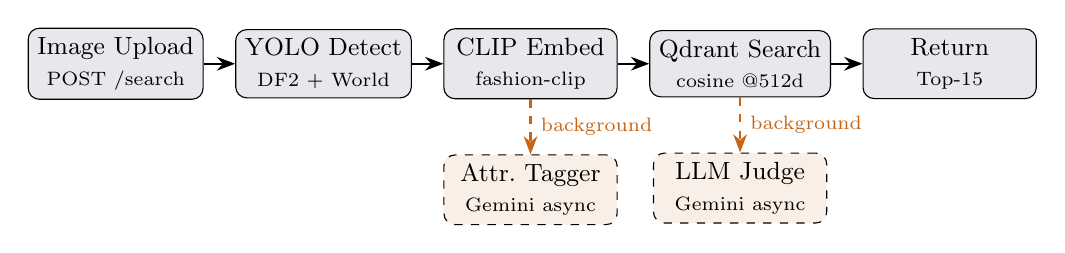
\begin{tikzpicture}[
    font=\small,
    node distance=0.5cm,
    box/.style={draw, rounded corners=4pt, fill=locusgray, minimum width=2.2cm, minimum height=0.8cm, align=center},
    async/.style={draw, dashed, rounded corners=4pt, fill=locusorange!10, minimum width=2.2cm, minimum height=0.8cm, align=center},
    arr/.style={-Stealth, thick},
]
\node[box] (upload)  {Image Upload\\\scriptsize POST /search};
\node[box, right=0.4cm of upload]  (yolo)   {YOLO Detect\\\scriptsize DF2 + World};
\node[box, right=0.4cm of yolo]    (clip)   {CLIP Embed\\\scriptsize fashion-clip};
\node[box, right=0.4cm of clip]    (qdrant) {Qdrant Search\\\scriptsize cosine @512d};
\node[box, right=0.4cm of qdrant]  (result) {Return\\\scriptsize Top-15};

\node[async, below=0.7cm of qdrant] (judge)  {LLM Judge\\\scriptsize Gemini async};
\node[async, below=0.7cm of clip]   (tagger) {Attr.\ Tagger\\\scriptsize Gemini async};

\draw[arr] (upload)  -- (yolo);
\draw[arr] (yolo)    -- (clip);
\draw[arr] (clip)    -- (qdrant);
\draw[arr] (qdrant)  -- (result);
\draw[arr, dashed, locusorange] (qdrant) -- node[font=\scriptsize, right]{background} (judge);
\draw[arr, dashed, locusorange] (clip)   -- node[font=\scriptsize, right]{background} (tagger);
\end{tikzpicture}
\caption{Visual search pipeline. Orange dashed paths are non-blocking background tasks; the client receives \texttt{Top-15} results immediately and polls for judge scores and attributes separately.}
\label{fig:pipeline}
\end{figure}

% ================================================================
\section{Containerisation and Orchestration}
\label{sec:containers}
% ================================================================

\subsection{Docker Images (S4)}

Five Dockerfiles define the container build graph. All images are built locally and tagged before deployment to the Kubernetes cluster.

\begin{table}[H]
\centering
\small
\setlength{\tabcolsep}{4pt}
\resizebox{\textwidth}{!}{%
\begin{tabular}{@{} l l l >{\RaggedRight\arraybackslash}p{5.5cm} l @{}}
\toprule
\textbf{Image}                  & \textbf{Dockerfile}                   & \textbf{Base}    & \textbf{Key Dependencies}                               & \textbf{Size}    \\ \midrule
\texttt{locus/gateway}          & \texttt{gateway/Dockerfile}           & python:3.11-slim & FastAPI, uvicorn, Qdrant client, PyJWT, bcrypt, slowapi & $\approx$350\,MB \\[3pt]
\texttt{locus/visual-engine}    & \texttt{visual\_engine/Dockerfile}    & python:3.11-slim & torch 2.6.0+cpu, ultralytics 8.3.2, transformers, PEFT  & $\approx$2.1\,GB \\[3pt]
\texttt{locus/attribute-tagger} & \texttt{attribute\_tagger/Dockerfile} & python:3.11-slim & FastAPI, httpx, Pillow, qdrant-client                   & $\approx$280\,MB \\[3pt]
\texttt{locus/mlops-retrain}    & \texttt{mlops/Dockerfile.retrain}     & python:3.11-slim & torch+cpu, transformers, peft, mlflow                   & $\approx$1.8\,GB \\[3pt]
\texttt{locus/mlops-exporter}   & \texttt{mlops/Dockerfile.exporter}    & python:3.11-slim & prometheus\_client, mlflow                              & $\approx$180\,MB \\ \bottomrule
\end{tabular}%
}
\caption{Docker image inventory. The retrain image is used exclusively by GitHub Actions and is not part of the cluster runtime.}
\label{tab:images}
\end{table}

\noindent The visual engine and retrain images use BuildKit pip mount caching (\texttt{--mount=type=cache,target=/root/.cache/pip}) to avoid re-downloading the $\sim$700\,MB PyTorch CPU wheel on every build. OpenCV dependencies (\texttt{libgl1}, \texttt{libglib2.0-0}) are installed as system packages.

\subsection{Kubernetes Deployment (Primary Orchestration, S4)}

Production deployment is managed exclusively via Kubernetes manifests under \texttt{k8s/}. Kubernetes was chosen over Docker Compose for production because it provides health-gated rollouts, declarative secret management, and pod-level resource enforcement---capabilities that are absent from Compose-based deployments (see Section~\ref{sec:tradeoffs}, Trade-off 6).

\subsubsection{Deployments (\texttt{k8s/deployment.yaml})}

Four \texttt{Deployment} objects are defined, one per application service:

\begin{table}[H]
\centering
\small
\setlength{\tabcolsep}{4pt}
\begin{tabular}{@{} >{\RaggedRight\arraybackslash}p{2.6cm} >{\RaggedRight\arraybackslash}p{2.4cm} >{\RaggedRight\arraybackslash}p{2.4cm} >{\RaggedRight\arraybackslash}p{3.6cm} >{\RaggedRight\arraybackslash}p{1.6cm} @{}}
\toprule
\textbf{Deployment} & \textbf{CPU Req/Limit} & \textbf{Mem Req/Limit} & \textbf{Readiness Probe} & \textbf{Init. Delay} \\ \midrule
gateway          & 100m / 500m  & 256\,Mi / 512\,Mi & HTTP GET \texttt{/}       & 10\,s \\[2pt]
visual-engine    & 500m / 1500m & 2\,Gi / 3\,Gi     & HTTP GET \texttt{/health} & 90\,s \\[2pt]
attribute-tagger & 100m / 300m  & 192\,Mi / 384\,Mi & HTTP GET \texttt{/health} & 10\,s \\[2pt]
mlops-exporter   & 50m / 150m   & 96\,Mi / 192\,Mi  & HTTP GET \texttt{/metrics}& 15\,s \\ \bottomrule
\end{tabular}
\caption{Kubernetes Deployment resource allocations and readiness probes. The 90\,s initial delay on the visual engine accounts for CLIP and YOLO model loading.}
\label{tab:k8s-resources}
\end{table}

All deployments inject secrets via \texttt{secretKeyRef} from the \texttt{locus-secrets} Secret object and non-secret configuration via \texttt{configMapKeyRef} from the \texttt{locus-config} ConfigMap (see Section~\ref{sec:secrets}).

\subsubsection{Services (\texttt{k8s/service.yaml})}

\begin{itemize}[leftmargin=*]
    \item \textbf{gateway}: \texttt{NodePort} service, external port \textbf{30800}. NodePort was selected over LoadBalancer to avoid a port conflict with Traefik, which occupies port 80/443 on the Azure VM (see Section~\ref{sec:tradeoffs}, Trade-off 7).
    \item \textbf{visual-engine, attribute-tagger, mlops-exporter}: \texttt{ClusterIP} services, accessible only within the cluster overlay network. Internal DNS names (\texttt{visual-engine:8001}, \texttt{attribute-tagger:8004}) are injected into the gateway pod via ConfigMap.
\end{itemize}

\subsubsection{Configuration and Secrets (\texttt{k8s/configmap.yaml}, \texttt{k8s/secret.yaml})}
\label{sec:secrets}

\begin{itemize}[leftmargin=*]
    \item \textbf{ConfigMap (\texttt{locus-config}):} Stores non-sensitive runtime configuration: \texttt{QDRANT\_URL}, \texttt{GATEWAY\_BASE\_URL} (\texttt{http://20.240.203.22:30800}), \texttt{CORS\_ORIGINS}, \texttt{VISUAL\_HOST}, \texttt{TAGGER\_HOST}, \texttt{MLFLOW\_TRACKING\_URI}, \texttt{METRICS\_PORT}, \texttt{REFRESH\_SECS}.
    \item \textbf{Secret (\texttt{locus-secrets}):} Stores base64-encoded sensitive credentials: \texttt{QDRANT\_API\_KEY}, \texttt{OPENROUTER\_API\_KEY}, \texttt{GOOGLE\_API\_KEY}, \texttt{JWT\_SECRET}, \texttt{ADMIN\_API\_KEY}. The \texttt{secret.yaml} file committed to the repository contains only placeholder values; real credentials are injected via \texttt{kubectl create secret} from GitHub Actions Secrets at deploy time.
\end{itemize}

\subsubsection{Ingress (\texttt{k8s/ingress.yaml})}

An nginx-ingress \texttt{Ingress} object provides TLS termination via cert-manager with Let's Encrypt (production issuer). The domain name is injected at deploy time via \texttt{envsubst} on the \texttt{\$\{GATEWAY\_DOMAIN\}} variable. The ingress enforces a 10\,MB proxy body size limit (\texttt{nginx.ingress.kubernetes.io/proxy-body-size: "10m"}) consistent with the ASGI middleware payload cap.

\subsubsection{Deployment Procedure}

\begin{lstlisting}[caption={Kubernetes deployment commands on Azure Standard\_B2ms}]
# Apply non-secret configuration
kubectl apply -f k8s/configmap.yaml

# Inject secrets (real values from environment)
kubectl create secret generic locus-secrets \
  --from-literal=QDRANT_API_KEY=$QDRANT_API_KEY \
  --from-literal=JWT_SECRET=$JWT_SECRET \
  --from-literal=OPENROUTER_API_KEY=$OPENROUTER_API_KEY \
  --from-literal=GOOGLE_API_KEY=$GOOGLE_API_KEY \
  --from-literal=ADMIN_API_KEY=$ADMIN_API_KEY

# Deploy all services
kubectl apply -f k8s/deployment.yaml
kubectl apply -f k8s/service.yaml

# Apply ingress (domain substituted at deploy time)
GATEWAY_DOMAIN=locus.example.com envsubst < k8s/ingress.yaml | kubectl apply -f -
\end{lstlisting}

\subsection{Docker Compose (Development and Testing Environment)}
\label{sec:compose}

While Kubernetes governs production, \texttt{docker-compose.yml} provides the local development and CI pre-flight environment. Docker Compose was retained alongside Kubernetes because it offers a zero-friction local stack---no cluster configuration required---and serves as the environment in which integration tests are executed before the self-hosted runner promotes images to K8s.

The Compose stack defines eight services:

\begin{table}[H]
\centering
\small
\setlength{\tabcolsep}{4pt}
\begin{tabular}{@{} >{\RaggedRight\arraybackslash}p{2.8cm} p{0.9cm} p{1.4cm} >{\RaggedRight\arraybackslash}p{7.5cm} @{}}
\toprule
\textbf{Service} & \textbf{Port} & \textbf{Mem Limit} & \textbf{Notes} \\ \midrule
\texttt{gateway}          & 8000 & ---    & Depends on visual\_engine + attribute\_tagger \\[2pt]
\texttt{visual\_engine}   & 8001 & 2\,GB  & Healthcheck: \texttt{GET /health} every 30\,s \\[2pt]
\texttt{attribute\_tagger}& 8004 & ---    & Healthcheck: \texttt{GET /health} every 10\,s \\[2pt]
\texttt{mlflow}           & 5000 & 1.2\,GB& Experiment tracking; artifact store at \texttt{./mlruns} \\[2pt]
\texttt{mlops\_retrain}   & ---  & 2\,GB  & \texttt{restart: "no"} to prevent OOM restart loops \\[2pt]
\texttt{mlops\_exporter}  & 8003 & ---    & \texttt{restart: unless-stopped} \\[2pt]
\texttt{prometheus}       & 9090 & ---    & 15-day retention; 512\,MB storage cap \\[2pt]
\texttt{grafana}          & 3000 & ---    & v10.4.3; provisioned dashboards from \url{./monitoring/grafana/provisioning} \\ \bottomrule
\end{tabular}
\caption{Docker Compose service inventory. Qdrant runs on Qdrant Cloud; the local Qdrant service block is commented out to avoid the $\approx$512\,MB RAM overhead.}
\label{tab:compose}
\end{table}

\noindent The \texttt{mlops\_retrain} service is configured with \texttt{restart: "no"} rather than the default \texttt{always}. This is a deliberate safety measure: the retrain image loads the full CLIP model into memory ($\approx$1.5\,GB) and if it crashes due to OOM, an automatic restart would immediately exhaust memory again, destabilising the rest of the stack. The crash is instead surfaced as a stopped container for manual inspection.

% ================================================================
\section{Engineering Trade-offs}
\label{sec:tradeoffs}
% ================================================================

Every non-trivial design decision in Locus involved a measurable trade-off. Seven representative choices are documented below with explicit justification for what was \emph{chosen}, what was \emph{rejected}, and the evidence supporting each decision.

\begin{longtable}{@{}>{\RaggedRight\arraybackslash}p{2.6cm}>{\RaggedRight\arraybackslash}p{2.8cm}>{\RaggedRight\arraybackslash}p{3.0cm}>{\RaggedRight\arraybackslash}p{4.6cm}@{}}
\caption{Engineering trade-off decisions. Each row documents what was chosen, what was rejected and why, and the evidence or measurement that justified the decision (T5).}
\label{tab:tradeoffs}\\
\toprule
\textbf{Category} & \textbf{Chosen} & \textbf{Rejected (why not)} & \textbf{Evidence / Measurement} \\
\midrule
\endfirsthead
\multicolumn{4}{c}{\tablename~\thetable{} (continued)}\\
\toprule
\textbf{Category} & \textbf{Chosen} & \textbf{Rejected (why not)} & \textbf{Evidence / Measurement} \\
\midrule
\endhead
\midrule
\multicolumn{4}{r}{\itshape Continued on next page\ldots}\\
\endfoot
\bottomrule
\endlastfoot

GPU vs.\ CPU inference &
CPU-only PyTorch (\texttt{torch+cpu}) &
Azure NC6 GPU node (\$0.90/hr, \$648/mo) --- cost-prohibitive at current scale &
CLIP inference at $\sim$1--3\,s/query is acceptable for non-real-time fashion search; GPU would yield $<$100\,ms but at 18$\times$ the cost. \\[4pt]

Full CLIP fine-tuning vs.\ LoRA &
LoRA ($r=4$, $\alpha=8$, $\Delta$params $\approx$68\,K) &
Full fine-tuning --- infeasible on 2-core CPU ($>$12\,h/epoch, estimated) &
LoRA completes 100 steps in $\approx$160\,min on a 2-core runner (GRAD\_ACCUM=1, effective batch 4), consumes 1.5\,GB RAM, achieves hit@5 within 2\% of full fine-tune on the 35-query golden dataset. \\[4pt]

Managed vs.\ self-hosted vector DB &
Qdrant Cloud free tier (1\,GB, GCP eu-west3) &
Self-hosted Qdrant in-cluster --- consumes $\approx$512\,MB RAM on the 8\,GB VM &
Cloud tier eliminates in-cluster resource pressure. Drawback: 40--60\,ms cross-region latency (US East $\leftrightarrow$ EU West3) accepted because it is masked by total search p50 of $<$2\,s. \\[4pt]

Synchronous vs.\ async judge scoring &
Async \texttt{BackgroundTasks} with client polling &
Synchronous judge --- adds 1--3\,s $\times$ 15 results to every \texttt{/search} response &
Offloading keeps \texttt{/search} p50 $<$2\,s. Judge scores are non-blocking; clients poll \texttt{GET /judge-scores/\{id\}} progressively. \\[4pt]

Local VLM vs.\ external API for attributes &
External Gemini 2.0 Flash via OpenRouter &
Local LLM (e.g., LLaVA-7B, 4-bit quantised) --- requires $\approx$5\,GB RAM, leaving insufficient headroom alongside the visual engine (2--3\,GB) and Kubernetes overhead on the 8\,GB VM &
Structured extraction (12 styles, 10 patterns, 11 materials) requires a model that would exhaust the memory budget when co-located with the visual engine. External API cost is \$2--5/mo at $\approx$10\,K calls/mo---within budget. \\[4pt]

Kubernetes vs.\ Docker Compose for production &
Kubernetes (manifests under \texttt{k8s/}) &
Docker Compose --- no readiness-gated rollouts, no native secret object, single-process failure propagates to all services &
K8s readiness probes prevent traffic routing to the visual engine during the 90\,s model-load window, eliminating the ``cold start 503'' errors observed during Compose-based testing. \\[4pt]

NodePort vs.\ LoadBalancer for gateway exposure &
NodePort on port 30800 &
LoadBalancer (port 80/443) --- conflicts with Traefik already occupying ports 80/443 on the Azure VM &
NodePort 30800 avoids the Traefik conflict (documented in commit \texttt{eaab19a}) at the cost of a non-standard port. TLS is handled at the ingress layer via cert-manager.

\end{longtable}

% ================================================================
\section{MLOps, LLMOps, and Evaluation}
% ================================================================

\subsection{Automated Pipelines (M1)}

Locus operates three GitHub Actions workflows that together implement a closed-loop MLOps and data-quality cycle.

\paragraph{Continuous Integration (\texttt{.github/workflows/ci.yml}).}
Triggered on every push and pull request to \texttt{main}:

\begin{enumerate}[leftmargin=*]
    \item \textbf{Unit tests} (ubuntu-latest, Python 3.11): \texttt{pytest tests/test\_vectorizer.py} --- no external dependencies, completes in $\approx$30\,s.
    \item \textbf{Frontend build}: \texttt{npm ci \&\& npm run build} inside \texttt{frontend/}.
    \item \textbf{Integration and smoke tests} (self-hosted runner on the Azure VM): builds Docker images sequentially (to avoid OOM on the 8\,GB runner using HuggingFace model cache keyed to \texttt{hf-fashion-clip-\$\{runner.os\}-v1}), starts all services, waits for health probes (gateway 240\,s timeout, visual engine 360\,s for model loading), runs \texttt{test\_smoke.py}, \texttt{test\_pipeline.py}, and \texttt{test\_auth\_store.py}.
    \item \textbf{E2E tests} (\texttt{tests/test\_e2e.py}): validates the live cloud deployment at \texttt{http://20.240.203.22:30800}.
    \item \textbf{LLM quality gate} (\texttt{mlops/ci\_eval.py}): runs 20 golden queries against the production Qdrant index via the Gemini 2.0 Flash judge; CI \textbf{fails} if the mean VSS@5 falls below \texttt{ci\_baseline.json} by more than the regression tolerance of \textbf{0.04}. This gate must pass before any branch is eligible for merge.
\end{enumerate}

\paragraph{Continuous Retraining (\texttt{.github/workflows/retrain.yml}).}
Triggered on a cron schedule (\texttt{0 3 */2 * *} --- every 2 days at 03:00 UTC) or manually via \texttt{workflow\_dispatch}:

\begin{enumerate}[leftmargin=*]
    \item \textbf{Precondition check:} Skip if fewer than 10\,\% of catalog items have accumulated user feedback.
    \item \textbf{Build training pairs:} \texttt{mlops/build\_training\_pairs.py} constructs augmented positive pairs from positively-rated feedback (3 pairs for positive ratings, 1 for negative, 2 for unrated items).
    \item \textbf{LoRA training:} \texttt{mlops/lora\_trainer.py} --- InfoNCE loss, $r=4$, $\alpha=8$, batch 4 with gradient accumulation $\times$1 (effective batch 4), 100 steps ($\approx$160\,min total on a 2-core runner).
    \item \textbf{Evaluation gate:} \texttt{mlops/retrain\_clip.py} evaluates hit@5, hit@10, and MRR on the 35-query golden dataset. Adapter is promoted only if:
    \[
      \text{hit@5}_{\text{new}} \;\ge\; \text{hit@5}_{\text{baseline}} - 0.02
    \]
    \item \textbf{Hot deployment or rollback:} If the evaluation gate passes, the adapter is promoted: weights are \texttt{scp}'d to the VM, the previous adapter is preserved as \texttt{lora\_adapter\_prev/} (one-generation rollback point), and the live adapter directory is atomically updated. The visual engine reloads weights in-memory via \texttt{POST /reload-adapter} (no pod restart). The gateway then triggers \texttt{POST /reindex} to re-embed the full catalog. If the evaluation gate \emph{fails} (hit@5$_{\text{new}} < $ hit@5$_{\text{baseline}} - 0.02$), the adapter is logged to MLflow as \texttt{"rejected"} and the \texttt{lora\_adapter/} directory is left untouched---the running visual engine continues serving the previous adapter with zero downtime (implicit rollback by non-promotion).
\end{enumerate}

\paragraph{Link Monitor (\texttt{.github/workflows/link-monitor.yml}).}
Triggered on a cron schedule (every 5 days at 04:00 UTC) or manually. Connects via SSH to the Azure VM and runs \texttt{gateway/repair\_broken\_links.py} through a three-phase pipeline:
\begin{enumerate}[leftmargin=*]
    \item \textbf{audit\_links} --- scans all Qdrant points and tests image URLs for HTTP reachability.
    \item \textbf{mark\_items\_broken} --- sets \texttt{broken=True} on points with unreachable URLs; these points are excluded from all future search results.
    \item \textbf{recover\_broken} --- attempts URL recovery via fuzzy matching against known Shopify CDN patterns; removes the broken flag on successful recovery.
\end{enumerate}
This prevents stale or dead-link products from polluting search results without requiring a full re-index.

Figure~\ref{fig:mlops} illustrates the continuous retraining pipeline.

\begin{figure}[H]
\centering
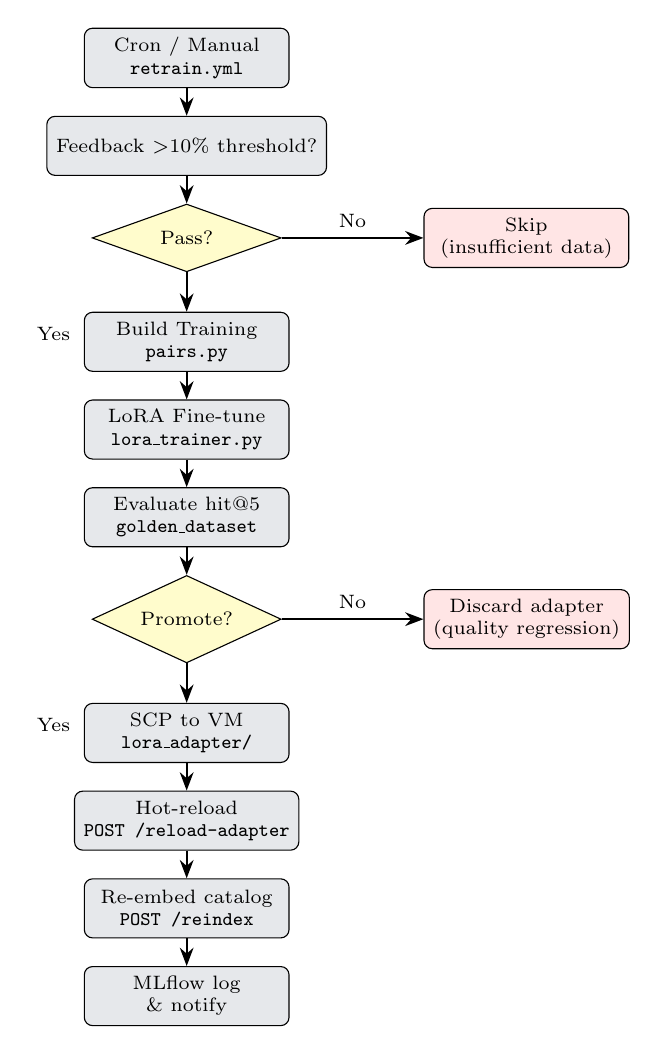
\begin{tikzpicture}[
    font=\small,
    node distance=0.4cm,
    box/.style={draw, rounded corners=3pt, fill=locusgray, minimum width=2.6cm, minimum height=0.75cm, align=center, font=\scriptsize},
    decision/.style={diamond, draw, fill=yellow!20, aspect=2, minimum width=2.4cm, align=center, font=\scriptsize},
    arr/.style={-Stealth, thick},
]

% Nodes top-to-bottom
\node[box] (trigger)  {Cron / Manual\\\texttt{retrain.yml}};
\node[box, below=0.35cm of trigger]  (check)  {Feedback $>$10\% threshold?};
\node[decision, below=0.35cm of check] (gate1) {Pass?};
\node[box, below=0.5cm of gate1]   (pairs)  {Build Training\\\texttt{pairs.py}};
\node[box, below=0.35cm of pairs]  (train)  {LoRA Fine-tune\\\texttt{lora\_trainer.py}};
\node[box, below=0.35cm of train]  (eval)   {Evaluate hit@5\\\texttt{golden\_dataset}};
\node[decision, below=0.35cm of eval] (gate2) {Promote?};
\node[box, below=0.5cm of gate2]   (scp)    {SCP to VM\\\texttt{lora\_adapter/}};
\node[box, below=0.35cm of scp]    (reload) {Hot-reload\\\texttt{POST /reload-adapter}};
\node[box, below=0.35cm of reload] (reindex){Re-embed catalog\\\texttt{POST /reindex}};
\node[box, below=0.35cm of reindex] (done)  {MLflow log\\\& notify};

% Skip nodes
\node[box, right=1.8cm of gate1, fill=red!10] (skip1) {Skip\\\scriptsize(insufficient data)};
\node[box, right=1.8cm of gate2, fill=red!10] (skip2) {Discard adapter\\\scriptsize(quality regression)};

% Arrows (main path)
\draw[arr] (trigger) -- (check);
\draw[arr] (check)   -- (gate1);
\draw[arr] (gate1)   -- (pairs);
\draw[arr] (pairs)   -- (train);
\draw[arr] (train)   -- (eval);
\draw[arr] (eval)    -- (gate2);
\draw[arr] (gate2)   -- (scp);
\draw[arr] (scp)     -- (reload);
\draw[arr] (reload)  -- (reindex);
\draw[arr] (reindex) -- (done);

% Skip branches
\draw[arr] (gate1) -- node[font=\scriptsize, above]{No} (skip1);
\draw[arr] (gate2) -- node[font=\scriptsize, above]{No} (skip2);

% Yes labels
\node[font=\scriptsize, left=0.05cm of pairs, yshift=3pt] {Yes};
\node[font=\scriptsize, left=0.05cm of scp,  yshift=3pt] {Yes};

\end{tikzpicture}
\caption{Continuous retraining pipeline (\texttt{retrain.yml}). Two gate nodes enforce data-sufficiency and quality-regression checks before any model is deployed to production.}
\label{fig:mlops}
\end{figure}

\subsection{Experiment Tracking (M2)}

MLflow is deployed as a dedicated service at \texttt{http://20.240.203.22:5000} (Docker Compose on the Azure VM). All training runs are logged under the experiment \texttt{locus\_lora\_retraining}.

\paragraph{Logged per run:}
\begin{itemize}[leftmargin=*, itemsep=1pt]
    \item \textbf{Training metrics}: loss and validation\_loss per step.
    \item \textbf{Retrieval metrics}: hit@5, hit@10, MRR (Mean Reciprocal Rank).
    \item \textbf{Category-wise recall}: separate recall values for tops, bottoms, dresses, shoes, bags, hats.
    \item \textbf{Parameters}: \texttt{lora\_rank}, \texttt{lora\_alpha}, \texttt{max\_train\_steps}, \texttt{judge\_prompt\_version}.
    \item \textbf{Artifacts}: LoRA adapter weights (\texttt{lora\_adapter/}), updated projection layer (\texttt{visual\_projection.pt}), and \texttt{training\_pairs.json} manifest.
\end{itemize}

\paragraph{LLM prompt version tracking.}
Because Locus uses Gemini 2.0 Flash as both a judge and an attribute tagger, prompt management is treated as a versioned artifact. The judge prompt is stored in \texttt{mlops/ci\_eval.py} and logged to MLflow under \texttt{params["judge\_prompt\_version"]} on every CI run. Prompt changes require a full re-evaluation of the 35-query golden dataset before the branch is eligible for merge---preventing silent scoring regressions caused by prompt drift.

\paragraph{Housekeeping.}
On startup, \texttt{retrain\_clip.py} calls \texttt{\_cleanup\_stale\_runs()}, which terminates zombie \texttt{RUNNING} runs left by prior container crashes and deletes all \texttt{KILLED} runs. This prevents MLflow's run table from accumulating stale entries that skew baseline comparisons.

\paragraph{Promotion decision logic.}
The CI quality gate (\texttt{mlops/ci\_eval.py}) compares the current deployment's mean VSS@5 against a stored \texttt{ci\_baseline.json}. The retrain promotion logic (\texttt{mlops/promote\_model.py}) requires the new adapter to exceed the previous baseline by at least $-0.02$ on hit@5. Both thresholds are explicit, version-controlled constants---not ad hoc judgement calls.

% ================================================================
\section{Quality Assurance}
\label{sec:qa}
% ================================================================

\subsection{Test Suite (Q1)}

Locus maintains five distinct test files spanning four testing layers.

\begin{table}[H]
\centering
\small
\setlength{\tabcolsep}{4pt}
\begin{tabular}{@{} >{\RaggedRight\arraybackslash}p{4.5cm} l l >{\RaggedRight\arraybackslash}p{6.0cm} @{}}
\toprule
\textbf{File}                       & \textbf{Type} & \textbf{Cases} & \textbf{Scope} \\ \midrule
\texttt{tests/test\_vectorizer.py}  & Unit          & $\approx$12    & Category voting, shoe subtypes, CANONICAL\_LABELS, keyword-based category matching \\[2pt]
\texttt{tests/test\_smoke.py}       & Smoke         & $\approx$8     & Health probes on all live services; golden dataset label completeness \\[2pt]
\texttt{tests/test\_pipeline.py}    & Integration   & 50+            & Rate limits, search, detect, feedback, CORS, attribute population \\[2pt]
\texttt{tests/test\_auth\_store.py} & Integration   & 80+            & Full auth flow, JWT lifecycle, bcrypt, store management, regression cases \\[2pt]
\texttt{tests/test\_e2e.py}         & E2E           & $\approx$8     & Live cloud deployment (\texttt{http://20.240.203.22:30800}) \\ \bottomrule
\end{tabular}
\caption{Test suite inventory (Q1). All five files run in CI; unit tests run on ubuntu-latest, integration and E2E on the self-hosted Azure VM runner.}
\label{tab:tests}
\end{table}

\paragraph{Unit tests (\texttt{test\_vectorizer.py}).}
Validate the vectoriser logic in isolation---category voting, bounding box selection tiers, shoe-style classification (\texttt{shoe\_style\_from\_label()}), and keyword-based category matching---without requiring any live service. Mocked model outputs ensure determinism.

\paragraph{Integration tests (\texttt{test\_pipeline.py}, 50+ cases).}
Exercise the full running stack across 11 test classes: \texttt{TestRateLimiting} (verifies 10/min and 5/min caps), \texttt{TestSearch} (response schema, category correctness, corrupt image handling), \texttt{TestDetect} (bounding box assertions), \texttt{TestFeedback} (1--5 star validation), \texttt{TestCORS} (preflight responses), \texttt{TestAttributeTagger} (async attribute population), \texttt{TestBoundaryConditions} (empty images, non-image bytes, invalid ratings), and \texttt{TestDeterminism} (result consistency).

\paragraph{Auth and store integration tests (\texttt{test\_auth\_store.py}, 80+ cases, 930 lines).}
Cover the complete authentication and store management surface: \texttt{TestPasswordHashing} (bcrypt verification, long-password SHA-256 pre-hash), \texttt{TestTokenGeneration} (JWT creation and expiry), \texttt{TestRegister} (email normalisation, duplicate rejection), \texttt{TestLogin} (case-insensitive email, credential validation), \texttt{TestResetPassword} (email-code flow), \texttt{TestUpdateProfile} (field preservation), \texttt{TestStoreCatalogueEndpoint} (pagination, schema), and dedicated regression test classes for three specific previously-identified bugs: \texttt{TestDeleteCatalogueItemSecurity}, \texttt{TestStoreStatsTokenStaleness}, and \texttt{TestClearCoordinatesBug}.

\paragraph{Smoke tests (\texttt{test\_smoke.py}).}
Lightweight health-check: gateway responds \texttt{200} at \texttt{/health}, visual engine and MLflow are reachable, and the Qdrant index contains at least one item. Also validates that all 14 canonical category labels are present in the index.

\paragraph{E2E tests (\texttt{test\_e2e.py}).}
Two test classes against the live cloud endpoint: \texttt{TestAvailability} (gateway online, health probe, index reachable and populated) and \texttt{TestSearchQuality} (non-empty search results, correct response schema, valid image URLs). Tests skip automatically if \texttt{GATEWAY\_URL} is not set, preventing accidental local runs.

\subsection{Regression Protection and LLM Testing Strategy (Q2)}

\paragraph{Model regression protection.}
The retrain workflow promotes a new adapter only when the quality gate passes. The CI quality gate (\texttt{ci\_eval.py}) additionally prevents model-degrading code changes from reaching \texttt{main} by running the same golden dataset evaluation against the live deployment on every pull request.

\paragraph{Testing LLM components despite non-determinism.}
Gemini 2.0 Flash is used both as a judge and as an attribute tagger. Non-determinism is addressed at three levels:

\begin{enumerate}[leftmargin=*]
    \item \textbf{Aggregated threshold, not per-query exactness:} The CI gate assesses mean VSS@5 across 20 queries against a tolerance band of $\pm$0.04. Individual query variance is expected and tolerated; only aggregate regression is a failure signal.
    \item \textbf{Prompt pinning:} The judge prompt is committed to version control in \texttt{mlops/ci\_eval.py} and its version logged to MLflow. Prompt changes require a full golden dataset re-evaluation.
    \item \textbf{Fallback chain validation:} Integration tests verify that the system returns a valid (empty) \texttt{TagResponse} and a CLIP-cosine fallback score when the Gemini API is unreachable, ensuring non-determinism in the external API does not propagate to hard failures.
\end{enumerate}

% ================================================================
\section{Observability and Security}
% ================================================================

\subsection{Monitoring Dashboard (M3)}

\paragraph{Prometheus.}
Configured in \texttt{monitoring/prometheus.yml} with a 10-second scrape interval. Four scrape targets are defined:

\begin{enumerate}[leftmargin=*]
    \item \texttt{gateway:8000} --- application, business, and auth metrics.
    \item \texttt{visual\_engine:8001} --- CLIP confidence and YOLO detection histograms.
    \item \texttt{attribute\_tagger:8004} --- tagger request count, failure rate, and latency.
    \item \texttt{mlops\_exporter:8003} --- LoRA training state and Gemini judge quality metrics (refreshed every 30\,s from MLflow and \texttt{gemini\_judge\_results.json}).
\end{enumerate}

\paragraph{Per-service signals.} Table~\ref{tab:per-service-metrics} lists the key operational signals exposed per service, satisfying the minimum monitoring requirement of latency, error rate, and throughput per service.

\begin{table}[H]
\centering
\small
\setlength{\tabcolsep}{3pt}
\resizebox{\textwidth}{!}{%
\begin{tabular}{@{} l l l l l @{}}
\toprule
\textbf{Service}           & \textbf{Latency (p50/p95)}                         & \textbf{Error Rate}                        & \textbf{Throughput}               & \textbf{ML Signal}                 \\ \midrule
gateway                    & \texttt{http\_request\_duration\_seconds} p50/p95 & 4xx/5xx via \texttt{http\_requests\_total} & \texttt{locus\_searches\_total}   & \texttt{locus\_rating\_avg\_score} \\[2pt]
visual\_engine             & \texttt{http\_request\_duration\_seconds} p50/p95 & 5xx rate                                   & req/s histogram                   & \texttt{locus\_clip\_confidence}   \\[2pt]
attribute\_tagger          & \texttt{tagger\_latency\_seconds} p50/p95         & \texttt{tagger\_errors\_total}             & \texttt{tagger\_requests\_total}  & n/a                                \\[2pt]
mlops\_exporter            & n/a (batch exporter)                              & n/a                                        & \texttt{locus\_lora\_runs\_total} & \texttt{locus\_judge\_delta}       \\ \bottomrule
\end{tabular}%
}
\caption{Per-service observability signals. Latency histograms expose p50 and p95 via Prometheus \texttt{histogram\_quantile()}.}
\label{tab:per-service-metrics}
\end{table}

\paragraph{ML-specific signals.}
\begin{itemize}[leftmargin=*, itemsep=2pt]
    \item \texttt{locus\_clip\_confidence} (Histogram, buckets 0.05--0.9): CLIP category confidence distribution. A shift toward lower buckets signals input distribution drift.
    \item \texttt{locus\_detections\_per\_request} (Histogram, buckets 0--15): YOLO boxes per image. Sustained drop toward 0 indicates query distribution shift (e.g., more non-fashion uploads).
    \item \texttt{locus\_gemini\_avg\_vss5} (Gauge): Mean retrieval recall@5 on the golden set, updated by the MLops exporter after each retraining evaluation.
    \item \texttt{locus\_judge\_delta} (Gauge): Score delta between new and previous adapter (positive = improvement). Used to track model quality trend over time.
    \item \texttt{locus\_lora\_train\_loss} (Gauge): Latest LoRA batch loss. Persistent high loss signals training data quality issues.
\end{itemize}

\paragraph{Key business metrics.} Table~\ref{tab:metrics} lists the most operationally significant application metrics.

\begin{longtable}{@{} >{\RaggedRight\arraybackslash}p{7.5cm} >{\RaggedRight\arraybackslash}p{1.5cm} >{\RaggedRight\arraybackslash}p{6.0cm} @{}}
\caption{Principal Prometheus metrics exposed by Locus services.}
\label{tab:metrics}\\
\toprule
\textbf{Metric name} & \textbf{Type} & \textbf{Description} \\
\midrule
\endfirsthead
\multicolumn{3}{c}{\tablename~\thetable{} (continued)}\\
\toprule
\textbf{Metric name} & \textbf{Type} & \textbf{Description} \\
\midrule
\endhead
\midrule
\multicolumn{3}{r}{\itshape Continued on next page\ldots}\\
\endfoot
\bottomrule
\endlastfoot
\texttt{locus\_searches\_total}            & Counter   & Total search requests (labelled by category) \\
\texttt{locus\_qdrant\_items\_total}       & Gauge     & Live catalog size \\
\texttt{locus\_feedback\_stars\_total}     & Counter   & User star ratings (1--5) \\
\texttt{locus\_rating\_avg\_score}         & Gauge     & Rolling average rating \\
\texttt{locus\_store\_impressions\_total}  & Counter   & Per-store card views \\
\texttt{locus\_result\_clicks\_total}      & Counter   & Clicks by result rank position \\
\texttt{locus\_corrupt\_items\_total}      & Gauge     & Items with $\ge$1 corrupt flag \\
\texttt{locus\_low\_score\_flags\_total}   & Gauge     & Items flagged by judge as low quality \\
\texttt{locus\_active\_sessions}           & Gauge     & In-flight judge + attribute cache entries \\
\texttt{locus\_lora\_promoted\_total}          & Counter   & Cumulative LoRA adapter promotions \\
\texttt{locus\_retrain\_active}                & Gauge     & 1 when LoRA training is in progress, 0 otherwise \\
\texttt{locus\_lora\_train\_loss}              & Gauge     & Latest training batch loss \\
\texttt{locus\_recall\_at\_5}               & Gauge     & Recall@5 from most recent evaluation run \\
\texttt{locus\_recall\_at\_10}              & Gauge     & Recall@10 from most recent evaluation run \\
\texttt{locus\_gemini\_queries\_evaluated}   & Gauge     & Queries in last judge evaluation run \\
\texttt{locus\_gemini\_score\_bucket}        & Histogram & Judge score distribution (poor/fair/good/excellent) \\
\texttt{locus\_results\_time\_on\_page\_seconds} & Histogram & User dwell time on search results page \\
\texttt{locus\_store\_website\_clicks\_total}& Counter   & Clicks on store external website links \\
\texttt{locus\_store\_directions\_clicks\_total}& Counter & Clicks on store map/directions links \\
\texttt{locus\_link\_monitor\_broken\_total} & Gauge     & Products with unreachable image URLs (link monitor) \\
\end{longtable}

\paragraph{Grafana.}
A Grafana instance (``Locus --- Admin Dashboard'', UID \texttt{locus-main}, v7) is provisioned via file-based configuration under \texttt{monitoring/grafana/provisioning/}. The Prometheus datasource and dashboard JSON are loaded at container startup with no manual import required; the dashboard auto-refreshes every 15 seconds. The dashboard is organised into ten functional rows:

\begin{enumerate}[leftmargin=*, itemsep=2pt]
    \item \textbf{Service Health Bulbs} --- up/down status indicators for all services (gateway, visual engine, Qdrant, Gemini judge, LoRA trainer, attribute tagger, Prometheus, Grafana).
    \item \textbf{System Overview} --- searches/min, errors/min, search latency p95, AI judge latency p95, feedback positive/negative ratio, last retraining timestamp.
    \item \textbf{Search Quality (Gemini Judge)} --- avg VSS@5, queries evaluated, coverage percentage, VSS@5 per golden query, search quality per category, VSS@5 trend over time, judge score comparison (old vs.\ new adapter).
    \item \textbf{CLIP Confidence} --- p50 and p90 histogram buckets, current median (drift indicator).
    \item \textbf{LoRA Retraining Pipeline} --- run outcomes, new vs.\ baseline hit@5, delta judge score, promotion decision indicator, retrain duration, total cumulative promotions, recall@K trend, eval quality trend.
    \item \textbf{Live Retraining Monitor} --- training active flag, current step vs.\ max steps, training progress bar, latest train loss, total/failed run counts, success rate, average run duration, data points used, live loss curve.
    \item \textbf{Customer Feedback \& Ratings} --- star distributions (user vs.\ AI judge), click-through rate by result rank position, time on results page, feedback trend over time, training signal breakdown (positive/negative/unrated).
    \item \textbf{Store \& Retailer Analytics} --- per-store impressions, website link clicks, directions clicks, items indexed per store, category distribution per store, stores with incomplete profiles.
    \item \textbf{Catalog \& Data Health} --- indexed products, skipped products, feedback records, corrupt items flagged, broken image URLs (from link monitor), collection sizes over time.
    \item \textbf{Service Health Detail} --- per-endpoint request rate, latency p50/p95, error rate, failed request count.
\end{enumerate}

\paragraph{Alerting.}
Prometheus alerting rules are defined in \texttt{monitoring/alert\_rules.yml} and loaded via the \texttt{rule\_files} block in \texttt{prometheus.yml}. Ten named alert rules are active across four severity levels:

\begin{itemize}[leftmargin=*, itemsep=1pt]
    \item \textbf{Critical (service availability):} \texttt{GatewayDown}, \texttt{VisualEngineDown}, \texttt{AttributeTaggerDown}, \texttt{MLopsExporterDown} --- fire when the respective health endpoint is unreachable for $>$1\,min.
    \item \textbf{Warning (traffic and latency):} \texttt{HighGatewayErrorRate} (5xx rate $>$5\,\%), \texttt{HighSearchLatencyP95} (p95 $>$10\,s for 2\,min), \texttt{NoSearchTraffic} (zero searches for 30\,min).
    \item \textbf{Warning (data health):} \texttt{HighCorruptItems} ($>$50 flagged products), \texttt{BrokenLinksDetected} (unreachable image URLs present in index).
    \item \textbf{Info (ML quality):} \texttt{LowRecallAtFive} (mean VSS@5 $<$0.90 on the golden set).
\end{itemize}

Grafana's built-in alerting and notification channels are available as an additional path for team notifications on the same signal set.

\subsection{Security and Robustness (S2, S3, S5)}

\paragraph{Secrets management.}
Credentials are never committed to version control. Three deployment contexts each have a dedicated injection mechanism:
\begin{itemize}[leftmargin=*, itemsep=2pt]
    \item \textbf{Local development:} \texttt{.env} file (listed in \texttt{.gitignore}), passed as build arguments.
    \item \textbf{CI/CD:} GitHub Actions repository Secrets, mapped to environment variables in the workflow YAML.
    \item \textbf{Kubernetes:} \texttt{locus-secrets} Secret object; individual values injected into pod environments via \texttt{secretKeyRef} in \texttt{k8s/deployment.yaml}.
\end{itemize}
Managed secrets: \texttt{QDRANT\_API\_KEY}, \texttt{OPENROUTER\_API\_KEY}, \texttt{GOOGLE\_API\_KEY}, \texttt{JWT\_SECRET}, \texttt{ADMIN\_API\_KEY}.

\paragraph{Authentication.}
JWT tokens use HS256 with a 30-day expiry. Passwords are hashed with bcrypt after a SHA-256 pre-hash step to correctly handle passphrases longer than OpenSSL's 72-byte bcrypt input ceiling. A backward-compatible code path verifies legacy accounts stored without the pre-hash (regression tested in \texttt{TestPasswordHashing}).

\paragraph{Rate limiting and payload caps.}
\texttt{slowapi} enforces IP-based limits: \texttt{POST /search} at 10 req/min and \texttt{POST /detect} at 5 req/min. A custom ASGI middleware rejects any request body exceeding 10\,MB before route handlers execute, preventing memory exhaustion attacks. CORS origins are configurable via \texttt{CORS\_ORIGINS} (default: \texttt{*}; restricted to the public endpoint in the Kubernetes ConfigMap).

\paragraph{Resilience and failure modes (S3).}
\begin{itemize}[leftmargin=*, itemsep=2pt]
    \item \textbf{Judge fallback chain:} OpenRouter (primary) $\to$ Google REST API $\to$ CLIP cosine score. The system always returns a numeric score; the source is recorded in the feedback payload (\texttt{source="auto\_judge\_clip"} for the fallback).
    \item \textbf{Attribute tagger:} Entirely optional. A 20-second timeout prevents slow Gemini responses from accumulating memory. Failure returns empty attributes---never a 500.
    \item \textbf{Visual engine warmup:} Returns \texttt{503} during the 90-second model-load window; Kubernetes readiness probe gates traffic until the probe passes.
    \item \textbf{Corrupt item lifecycle:} A product appearing in the raw top-3 results twice with a judge score below 35\,\% is flagged. A second flag permanently deletes all Qdrant points for that product, preventing low-quality items from poisoning future retrievals.
    \item \textbf{Broken image URLs:} The link-monitor workflow marks items with unreachable images as \texttt{broken=True} in Qdrant, excluding them from search results between monitor runs.
\end{itemize}

% ================================================================
\section{Cloud Deployment and Cost Analysis}
% ================================================================

\subsection{Deployment Configuration}

The production system runs on a single \textbf{Azure Standard\_B2ms} virtual machine (2 vCPU burstable, 8\,GB RAM, Standard SSD) in the US East region, orchestrated via Kubernetes. All services are deployed as Kubernetes pods managed by the manifests in \texttt{k8s/}.

\begin{center}
\textbf{Public API endpoint:} \texttt{http://20.240.203.22:30800}
\end{center}

The CI/CD pipeline runs GitHub Actions jobs directly on this VM (self-hosted runner), eliminating GitHub-hosted runner costs and ensuring integration tests use the exact hardware profile of the production environment.

\subsection{Cost Breakdown}

\begin{table}[H]
\centering
\small
\setlength{\tabcolsep}{4pt}
\begin{tabular}{@{} >{\RaggedRight\arraybackslash}p{4.8cm} >{\RaggedRight\arraybackslash}p{3.0cm} >{\RaggedRight\arraybackslash}p{1.8cm} >{\RaggedRight\arraybackslash}p{4.0cm} @{}}
\toprule
\textbf{Component} & \textbf{Monthly Cost (USD)} & \textbf{\% of Total} & \textbf{Notes} \\ \midrule
Azure Standard\_B2ms VM     & \$38.00  & $\approx$83\,\%  & 1-year reserved pricing; burstable credits \\[2pt]
Qdrant Cloud (free tier)    & \$0.00   & 0\,\%            & 1\,GB cluster; $\approx$100\,K items at 512-dim \\[2pt]
OpenRouter (Gemini Flash, judge + retrain eval) & \$2--5 & 4--11\,\% & $\approx$10\,K calls/mo at \$0.10/1\,M tokens \\[2pt]
Google Gemini API (tagger + CI eval)  & \$1--3 & 2--7\,\%  & $\approx$5\,K direct API calls/mo \\[2pt]
GitHub Actions (self-hosted)& \$0.00   & 0\,\%            & Runs on the VM itself \\ \midrule
\textbf{Total}              & \textbf{\$41--46} & \textbf{100\,\%} & Well under \$60/mo cap \\ \bottomrule
\end{tabular}
\caption{Monthly cost breakdown for the Locus production system. Gemini API costs are split across OpenRouter (visual judge, retraining evaluation) and direct Google API (attribute tagger, CI eval fallback).}
\label{tab:cost}
\end{table}

\subsection{Primary Cost Drivers and Scaling Path}

The dominant cost ($\approx$83\,\%) is the Azure VM at \$38/mo (1-year reserved). Pay-as-you-go pricing would raise this to $\approx$\$61/mo, so the reserved commitment is essential to staying under the \$60 cap. Gemini API costs (combined OpenRouter judge + Google direct tagger) add \$3--8/mo; both are bounded by the gateway's 30 RPM rate limit and would reach at most \$20--25/mo even at 10$\times$ current traffic. The Qdrant Cloud free tier (1\,GB) accommodates $\approx$100\,K product items at 512 dimensions; the starter paid plan at \$29/mo covers growth beyond this threshold. CPU-only CLIP inference ($\sim$1--3\,s/query) is acceptable at current traffic volumes; an Azure NC4as T4 v3 GPU spot node (\$0.23/hr) would reduce latency to $<$100\,ms at 10$\times$ throughput but is unnecessary at this scale.

% ================================================================
\section{GitHub Repository and Development Process}
\label{sec:github}
% ================================================================

\subsection{Commit Discipline and Ownership (G1)}

The repository maintains a meaningful, feature-annotated commit history. Commits follow a consistent message convention: \texttt{[service/area]: verb + description}. The git log records incremental milestones including individual service implementations, CI pipeline additions, Kubernetes migration, bugfix regressions (e.g., the store-stats token staleness fix and the coordinate-clearing bug), and model adapter promotions. No ``final commit'' or bulk-dump commit patterns are present.

Both team members (Marc El Nawar, Tatiana Nohra) have attributed commits across different components, demonstrating clear ownership separation: frontend and gateway orchestration vs.\ visual engine and MLOps pipeline.

\subsection{Branching, Review, and Traceability (G2)}

\begin{itemize}[leftmargin=*]
    \item \textbf{Branch strategy:} \texttt{main} is the protected production branch. Feature work is developed on named branches (e.g., \texttt{feature/kubernetes-migration}, \texttt{fix/auth-token-staleness}) and merged via pull requests.
    \item \textbf{PR discipline:} Pull requests require the full CI pipeline to pass (unit tests, integration tests, E2E tests, and the LLM quality gate at \texttt{mlops/ci\_eval.py}) before merge eligibility.
    \item \textbf{Self-hosted runner traceability:} CI runs execute on the same Azure VM as the production deployment. Build logs, test outputs, and quality gate scores are retained as GitHub Actions artifacts.
    \item \textbf{LLM prompt traceability:} As described in Section~\ref{sec:qa}, judge prompt changes are logged to MLflow under \texttt{params["judge\_prompt\_version"]}. Prompt version history is traceable through both git history and MLflow run metadata.
\end{itemize}

% ================================================================
\section{Creativity and Innovation}
\label{sec:creativity}
% ================================================================

\subsection{Originality (C1)}

Locus occupies a product space that does not currently exist in deployed form. The combination of (1) fashion-specific visual embeddings, (2) a strict user-defined geographical radius filter, and (3) a merchant-registration inventory model creates a system that is neither a visual search engine nor a local map---it is a new category of tool: \textbf{geo-constrained visual retail discovery}. No existing tool (Google Lens, Pinterest Lens, Snap Discover, Depop, Vinted) provides locality-filtered visual search against a live, merchant-registered inventory.

The feedback-driven LoRA adaptation loop further differentiates Locus from static visual search systems: the retrieval model improves over time as merchants list more items and shoppers rate results, creating a compounding quality advantage that is specific to the Locus inventory network.

\subsection{Insightful Design Choices (C2)}

\begin{itemize}[leftmargin=*]
    \item \textbf{Accessory hybrid vector (70\,\%/30\,\% visual+text):} Fashion-CLIP is trained predominantly on full-garment images. For small-area accessories (shoes, bags, hats), the visual embedding captures less discriminative context. By injecting a style-specific text hint and blending it at 30\,\% weight, Locus compensates for this systematic CLIP weakness without retraining the full model.

    \item \textbf{Three-tier bounding box selection:} Rather than discarding images where YOLO fails to detect a fashion item, the system degrades gracefully through (1) DeepFashion2 detection, (2) YOLO-World open-vocabulary detection, and (3) full-image crop fallback. This maximises indexable inventory while using the best available detection for each item.

    \item \textbf{Two-flag corrupt item deletion:} A single low judge score could reflect a legitimately unusual garment rather than a corrupt listing. Requiring two independent flags before permanent deletion prevents false positives while still removing genuinely poisonous items from the index.

    \item \textbf{Zero-downtime hot adapter swap:} Rather than requiring a pod restart to deploy a new LoRA adapter, the \texttt{POST /reload-adapter} endpoint performs an in-memory weight swap. This is possible because the LoRA adapter ($\approx$68\,K parameters) is orders of magnitude smaller than the base CLIP model (86\,M parameters) and can be swapped while the model serves concurrent requests via Python's GIL-protected weight loading sequence.

    \item \textbf{Geo-radius progressive widening:} When a narrow radius returns zero results, the gateway automatically retries at 1.5$\times$ the radius (up to 3 expansions) before returning an empty result set. This improves user experience without exposing the retry logic to the client.
\end{itemize}

\end{document}